% Copyright 2004 by Till Tantau <tantau@users.sourceforge.net>.
%
% In principle, this file can be redistributed and/or modified under
% the terms of the GNU Public License, version 2.
%
% However, this file is supposed to be a template to be modified
% for your own needs. For this reason, if you use this file as a
% template and not specifically distribute it as part of a another
% package/program, I grant the extra permission to freely copy and
% modify this file as you see fit and even to delete this copyright
% notice. 

\documentclass{beamer}

% There are many different themes available for Beamer. A comprehensive
% list with examples is given here:
% http://deic.uab.es/~iblanes/beamer_gallery/index_by_theme.html
% You can uncomment the themes below if you would like to use a different
% one:
%\usetheme{AnnArbor}
%\usetheme{Antibes}
%\usetheme{Bergen}
%\usetheme{Berkeley}
%\usetheme{Berlin}
%\usetheme{Boadilla}
%\usetheme{boxes}
%\usetheme{CambridgeUS}
%\usetheme{Copenhagen}
%\usetheme{Darmstadt}
%\usetheme{default}
%\usetheme{Frankfurt}
%\usetheme{Goettingen}
%\usetheme{Hannover}
%\usetheme{Ilmenau}
%\usetheme{JuanLesPins}
%\usetheme{Luebeck}
\usetheme{Madrid}
%\usetheme{Malmoe}
%\usetheme{Marburg}
%\usetheme{Montpellier}
%\usetheme{PaloAlto}
%\usetheme{Pittsburgh}
%\usetheme{Rochester}
%\usetheme{Singapore}
%\usetheme{Szeged}
%\usetheme{Warsaw}
\usepackage{graphicx} % Allows including images
\usepackage{booktabs} % Allows the use of \toprule, \midrule and \bottomrule in tables
\usepackage{subfig}
\usepackage[justification=centering]{caption}
\usepackage{lastpage}
\usepackage{tikz}
\usepackage{xcolor}
\usepackage{color}
\usepackage{float}
\def\Put(#1,#2)#3{\leavevmode\makebox(0,0){\put(#1,#2){#3}}}
\colorlet{beamer@blendedblue}{green!30!black}

\title{MorphoBoid Group}

% A subtitle is optional and this may be deleted
%\subtitle{Optional Subtitle}

%\author{F.~Author\inst{1} \and S.~Another\inst{2}}
% - Give the names in the same order as the appear in the paper.
% - Use the \inst{?} command only if the authors have different
%   affiliation.

%\institute[Universities of Somewhere and Elsewhere] % (optional, but mostly needed)
%{
%  \inst{1}%
%  Department of Computer Science\\
%  University of Somewhere
%  \and
%  \inst{2}%
%  Department of Theoretical Philosophy\\
%  University of Elsewhere}
% - Use the \inst command only if there are several affiliations.
% - Keep it simple, no one is interested in your street address.

%\date{Talence, 2017}
\date{}
% - Either use conference name or its abbreviation.
% - Not really informative to the audience, more for people (including
%   yourself) who are reading the slides online

% This is only inserted into the PDF information catalog. Can be left
% out. 

% If you have a file called "university-logo-filename.xxx", where xxx
% is a graphic format that can be processed by latex or pdflatex,
% resp., then you can add a logo as follows:

% \pgfdeclareimage[height=0.5cm]{university-logo}{university-logo-filename}
% \logo{\pgfuseimage{university-logo}}

% Delete this, if you do not want the table of contents to pop up at
% the beginning of each subsection:

% Let's get started
\setlength{\fboxrule}{0pt}
\begin{document}

\begin{frame}[t]
%\Put(70,-190){
\includegraphics[scale=0.4]{images/UB}}
\Put(270,-280){
\includegraphics[scale=1.8]{images/labri}}
  \titlepage
  \Put(0,150){
	  \fbox{
	  	\parbox{\textwidth}
	  	{
			Methods:
		\begin{enumerate}
  	\item Image processing:
	\begin{itemize}
		\item Segmentation of shape,
		\item Image registration,
		\item SIFT patch computing to set points of interest.
	\end{itemize}
	\item Deep learning:
	\begin{itemize}
		\item Convolutional neural networks (CNN) for classifying the images,
		\item CNN to predict the positions of the landmarks,
		\item Tools: Caffe, Theano, Lasagne.
	\end{itemize}
  \end{enumerate}	  	
	  	}
	  }
  }
  %Methods:
  %\begin{enumerate}
  %	\item Image processing:
%	\begin{itemize}
%		\item Segmentation of shape,
%		\item Image registration,
%		\item SIFT patch computing to set points of interest.
%	\end{itemize}
%	\item Deep learning:
%	\begin{itemize}
%		\item Convolutional neural networks (CNN) for classifying the images,
%		\item CNN to predict the positions of the landmarks,
%		\item Tools: Caffe, Theano, Lasagne.
%	\end{itemize}
 % \end{enumerate}
  
\end{frame}

%\begin{frame}{Outline}
%  \tableofcontents
  % You might wish to add the option [pausesections]
%\end{frame}

%\begin{frame}[t]{Application to Beetle collection: automatisation of landmarks setting}
  
%  \Put(259,-190){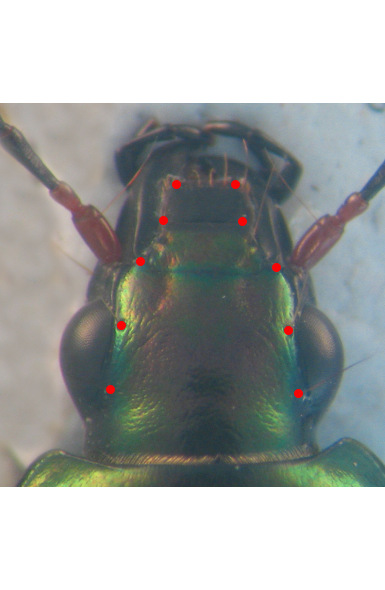
\includegraphics[scale=0.22]{images/tete}}
%\Put(255,-370){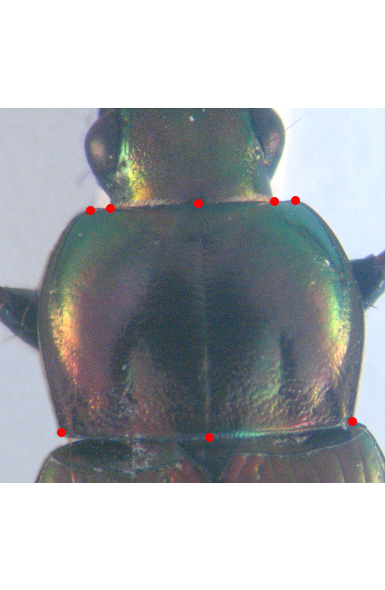
\includegraphics[scale=0.22]{images/pronotum}}
%\Put(162,-293){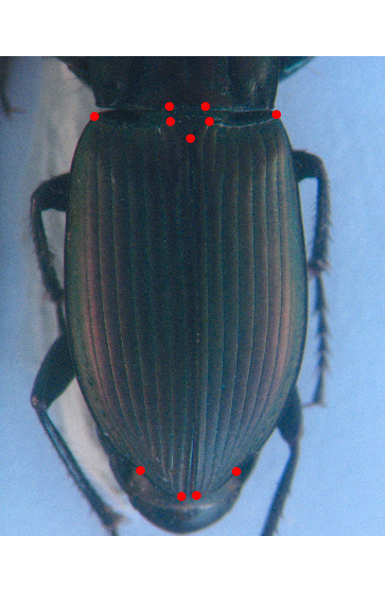
\includegraphics[scale=0.22]{images/elytre}}
%\Put(10,-270){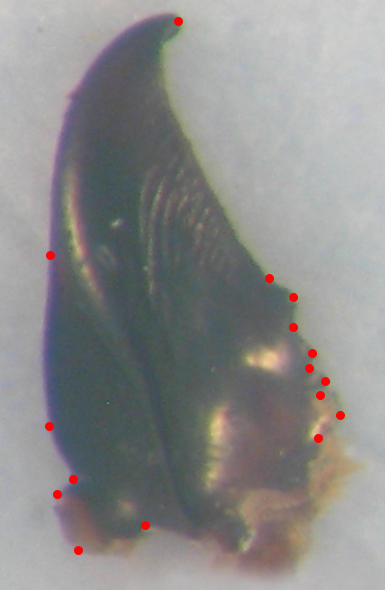
\includegraphics[scale=0.18]{images/mgmo}}
%\Put(80,-270){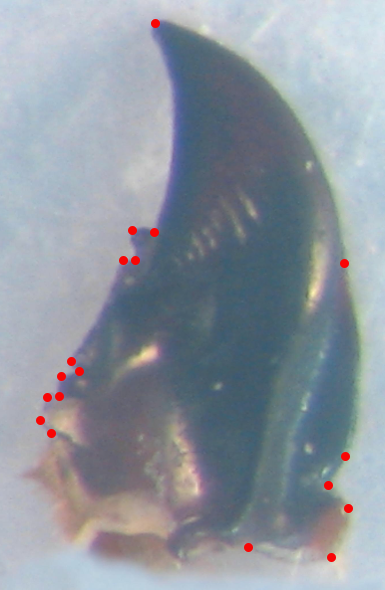
\includegraphics[scale=0.18]{images/mdmo}}
%\end{frame}
\begin{frame}[t]{Application to Beetle collection: automatisation of landmarks setting}
  
  \Put(70,-430){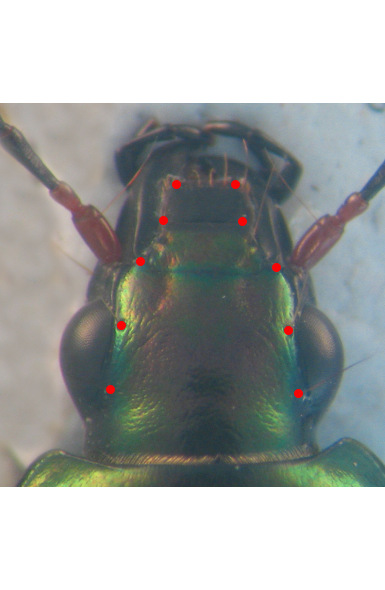
\includegraphics[scale=0.22]{images/tete}}
\Put(180,-430){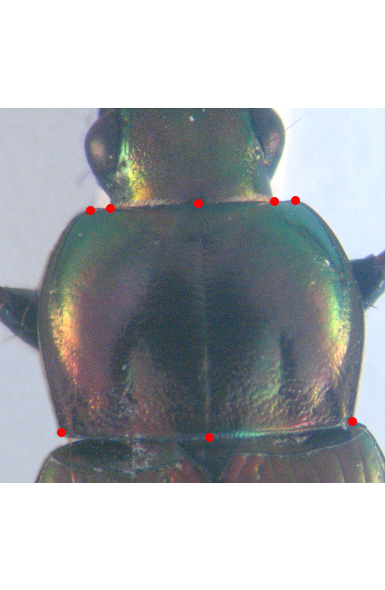
\includegraphics[scale=0.22]{images/pronotum}}
\Put(230,-223){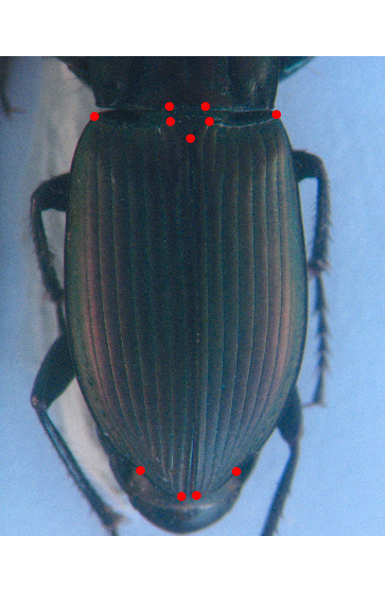
\includegraphics[scale=0.24]{images/elytre}}
\Put(10,-200){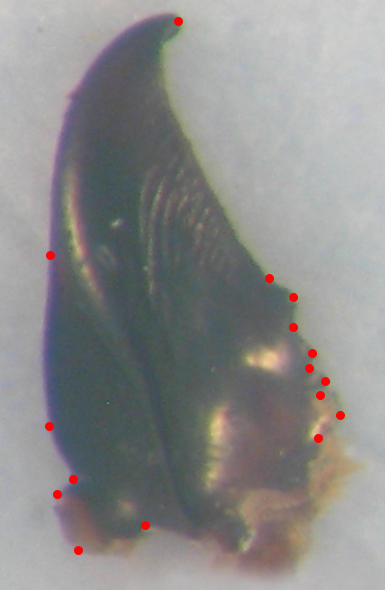
\includegraphics[scale=0.2]{images/mgmo}}
\Put(115,-200){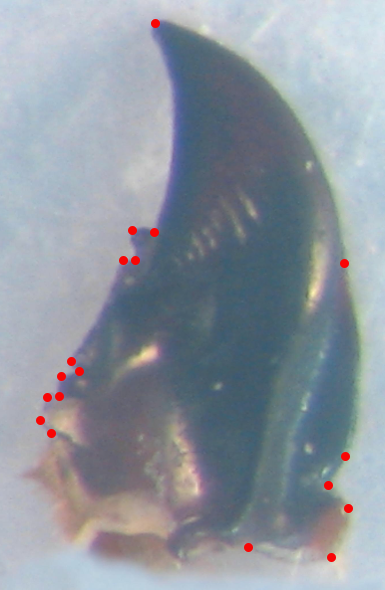
\includegraphics[scale=0.2]{images/mdmo}}
\end{frame}
% You can reveal the parts of a slide one at a time
% with the \pause command:
\begin{frame}[t]{Application to Papyrus: fragments matching}

  \Put(15,-330){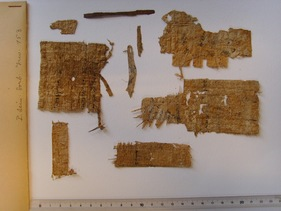
\includegraphics[scale=1]{images/p1}}
  \Put(250,-100){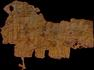
\includegraphics[scale=1.2]{images/p12}}
  \Put(225,-230){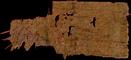
\includegraphics[scale=1.2]{images/p13}}
  \Put(240,-410){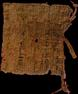
\includegraphics[scale=1.2]{images/p11}}
\end{frame}
\begin{frame}[t]{Application to observatory of Vietnam's heritages: images classification}	
	\Put(8,-360){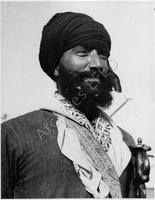
\includegraphics[scale=0.5]{images/h1}}
  \Put(120,-140){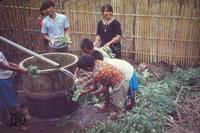
\includegraphics[scale=0.5]{images/h2}}
  \Put(0,-150){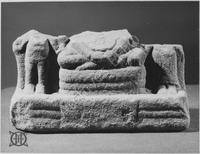
\includegraphics[scale=0.5]{images/h3}}
  \Put(230,-140){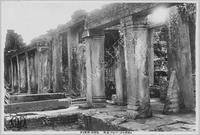
\includegraphics[scale=0.5]{images/h4}}
  \Put(80,-360){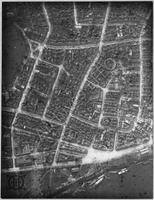
\includegraphics[scale=0.5]{images/h5}}
  \Put(160,-360){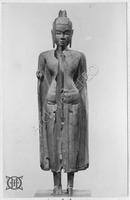
\includegraphics[scale=0.5]{images/h8}}
  \Put(225,-330){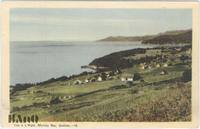
\includegraphics[scale=0.5]{images/h6}}
\end{frame}

% Placing a * after \section means it will not show in the
% outline or table of contents.

%\begin{frame}[t]{Methods}
%	Image processing:
%	\begin{itemize}
%		\item Segmentation of shape,
%		\item Image registration,
%		\item SIFT patch computing to set points of interest.
%	\end{itemize}
%	Deep learning:
%	\begin{itemize}
%		\item Convolutional neural networks (CNN) to train for classifying the images,
%		\item CNN to predict the positions of the landmarks,
%		\item Tools: Caffe, Theano, Lasagne.
%	\end{itemize}
%\end{frame}
\begin{frame}[t]{Peoples}	
	\begin{minipage}[t]{\textwidth}
		\begin{minipage}[t]{0.45\textwidth}
		\textbf{Team}
		\begin{enumerate}
			\item Marie BEURTON-AIMAR
			\item Jean-Pierre SALMON
			\item Nicholas JOURNET
			\item Van Linh LE
			\item Xuan Thanh PHAM
			\item Manh Tu VU
		\end{enumerate}
		\end{minipage}%
		\hspace{0.05\textwidth}
		\begin{minipage}[t]{0.5\textwidth}
		\textbf{Collaborations} - LaBRI		
		\small{
		\begin{enumerate}
			\item Team \textit{Distributed Algorithms}:\\ Akka ZEMMARI
			\item Team \textit{MABioVis}: Joris SANSEN
		\end{enumerate}}
		\textbf{Collaborations} - Others
		\small{
		\begin{enumerate}
			\item \textit{INRA Rennes}: Nicolas PARISEY
			\item \textit{AUSONIUS}:\\Marie-Pierre CHAUFRAY
			\item \textit{L3i La Rochelle}: Muriel VISANI
			\item \textit{Heritage Observatory}:\\Daniel CAUNE
			\item \textit{ICube, Strasbourg}:\\Adrien KRAHENBUHL
		\end{enumerate}
		}
		\end{minipage}
	\end{minipage}
	
	
\end{frame}


\end{document}


